\RequirePackage{plautopatch}
\documentclass[report,a4paper,uplatex,dvipdfmx,11pt]{jsbook}
\usepackage[dvipdfmx]{graphicx,color}
\usepackage{amsmath, amssymb,  latexsym, mathtools}
\usepackage{amsthm}
\usepackage{amsfonts}
\usepackage{bm} %数式中でボールド体も斜体にする。\bm{a}と書けば、斜体ボールドのaが書ける
\usepackage{midpage}
\usepackage[dvipdfmx]{graphicx,color}
\usepackage[hyphens]{url}
\usepackage[sort,compress,numbers]{natbib} % apsrev4-2ja.bstを使うのに必要
\usepackage{doi}
\usepackage{cleveref}
\usepackage{tocloft}
\usepackage{autonum}
\usepackage{hyperref}
\usepackage{pxjahyper}
\usepackage{xcolor}
\hypersetup{
  colorlinks=true,
  bookmarksnumbered=true,
  citecolor=blue,
  linkcolor=violet,
  urlcolor=blue,
  }

\crefname{definition}{}{}
\crefname{example}{}{}
\crefname{theorem}{}{}
\crefname{lemma}{}{}
\crefname{corollary}{}{}
\crefname{remark}{}{}
\crefname{proposition}{}{}
\crefname{proof}{}{}
\crefname{figure}{}{}
\crefname{chapter}{}{}
\crefname{section}{}{}
\crefname{subsection}{}{}
\crefname{equation}{式}{式}

\creflabelformat{definition}{#2\textbf{Definition} \textbf{#1}#3}
\creflabelformat{example}{#2\textbf{Example} \textbf{#1}#3}
\creflabelformat{theorem}{#2\textbf{Theorem} \textbf{#1}#3}
\creflabelformat{lemma}{#2\textbf{Lemma} \textbf{#1}#3}
\creflabelformat{corollary}{#2\textbf{Corollary} \textbf{#1}#3}
\creflabelformat{remark}{#2\textbf{Remark} \textbf{#1}#3}
\creflabelformat{proposition}{#2\textbf{Proposition} \textbf{#1}#3}
\creflabelformat{proof}{#2\textit{Proof} \textbf{#1}#3}
\creflabelformat{figure}{#2Figure #1#3}
\creflabelformat{chapter}{#2第#1章#3}
\creflabelformat{section}{#2第#1節#3}
\creflabelformat{subsection}{#2第#1小節#3}

\renewcommand{\figurename}{Figure }

% 参考文献の書式の設定-----------------------------------------------------------------
% \bibliographystyle{apsrev4-2ja} % アメリカ物理学会(APS)の標準のbibtexスタイルファイル
% \bibliographystyle{junsrt} % 文献のタイトルまで表示したい場合はこちらを使う
% \bibliographystyle{jplain}
\bibliographystyle{amsplain}
% -------------------------------------------------------------------------------------


% 余白の設定をするためのパッケージ------------------------------
%\usepackage[pass]{geometry}
%\usepackage{bxpapersize}
% --------------------------------------------------------------


% 章見出しの上の余白を小さくする--------------------------------
\usepackage{etoolbox}
\makeatletter
\patchcmd{\@makechapterhead}{\vspace*{2\Cvs}}{}{}{}
\patchcmd{\@makeschapterhead}{\vspace*{2\Cvs}}{}{}{}
\makeatother
\renewcommand{\cftbeforetoctitleskip}{0pt}
% --------------------------------------------------------------


% 目次のフォントについて----------------------------------------------------
% 1. 見出しの文字を明朝体にする(太字にはならない)
%\renewcommand{\headfont}{\mcfamily}

% 2. 明朝体の太字を使う場合は、
%\usepackage[deluxe]{otf}
%\renewcommand{\headfont}{\mcfamily\bfseries}

% 3. 見出し全てではなく、目次のフォントのみ変更する場合は、
\renewcommand{\cftchapnumwidth}{3.8em}
\renewcommand{\cftchapfont}{\mcfamily}
\renewcommand{\cftchappagefont}{\rmfamily}
% --------------------------------------------------------------------------


% 目次に参考文献を表示する ---------------------------------------
\makeatletter
\renewenvironment{thebibliography}[1]{%
 \bibsection\parindent \z@\bibpreamble\bibfont\list
   {\@biblabel{\arabic{NAT@ctr}}}{\@bibsetup{#1}%
   \addcontentsline{toc}{chapter}{\bibname}%
    \setcounter{NAT@ctr}{0}}%
    \ifNAT@openbib
      \renewcommand\newblock{\par}
    \else
      \renewcommand\newblock{\hskip .11em \@plus.33em \@minus.07em}%
    \fi
    \sloppy\clubpenalty4000\widowpenalty4000
    \sfcode`\.=1000\relax
    \let\citeN\cite \let\shortcite\cite
    \let\citeasnoun\cite
 }{\def\@noitemerr{%
  \PackageWarning{natbib}
     {Empty `thebibliography' environment}}%
  \endlist\vskip-\lastskip}
 \let\bibfont\relax
\makeatother
% ----------------------------------------------------------------


% 卒論で、図をページ数に含めたくないときに用いる図・表環境-------------
\newenvironment{clearpagefigure}
{\newpage
  \begin{midpage}
  \begin{figure}[htbp]
  \centering
  \thispagestyle{empty}
  \addtocounter{page}{-1}}
{\end{figure}
  \end{midpage}
  \newpage}

\newenvironment{clearpagetable}
{
\clearpage
\begin{table}
\centering
\thispagestyle{empty}
\addtocounter{page}{-1}
}
{\end{table}}
% ---------------------------------------------------------------------


\setcounter{tocdepth}{2} % 目次にどのレベルのセクションまで反映させるか。2だとsubsectionまで。

\allowdisplaybreaks % 数式の途中での改ページを許す

%---------------------------------------------
\newtheoremstyle{myDefinition}%   % スタイル名
    {11pt}%b                     % 上部スペース
    {16pt}%                      % 下部スペース
    {}%              % 本文フォント
    {}%                      % 1行目のインデント量
    {\bfseries}%             % 見出しフォント
    {.}%                     % 見出し後の句読点
    {11pt}%                     % 見出し後のスペース
    {\thmname{#1}\thmnumber{ #2}\thmnote{ (#3)}}

\theoremstyle{myDefinition}
\newtheorem{definition}{Definition}[section]
\theoremstyle{myDefinition}
\newtheorem{theorem}[definition] {Theorem}
\theoremstyle{myDefinition}
\newtheorem{proposition}[definition] {Proposition}
\theoremstyle{myDefinition}
\newtheorem{lemma}[definition] {Lemma}
\theoremstyle{myDefinition}
\newtheorem{corollary}[definition] {Corollary}
\theoremstyle{myDefinition}
\newtheorem{example}[definition] {Example}
\theoremstyle{myDefinition}
\newtheorem{remark}[definition] {Remark}



\title{パズルルールの自動作成を目指した数学的考察}
\author{前田樹}
\date{\today}

\begin{document}

\maketitle

\frontmatter
\chapter*{{\rm \bf Abstract}}\label{chapter:Abstract}
最適化を好む現代社会においては, エンターテイメントもその対象である. 技術の発展とともに, 人々は冗長なエンターテイメントを忌避するようになり, より短く, より楽しく, より強い刺激を求めるようになった. 無駄を徹底的に省いた娯楽に私はどこかもの寂しさを感じずにはいられない. 私たちが幼少期の頃に触れた娯楽は, 無駄の多い, 冗長なものばかりだった. そうすることでしか得られないカタルシスがあったのだろう. その媒体が私にとってはパズルだった. だが, パズルは時代の波に追いやられ, いまや本屋の棚の片隅で存在感を希薄にしているのである. ただ, 私は面白いパズルがもう一度解きたい. その一心で, 私自身が新しいパズルルールを生み出し, 自分の手で面白いパズルを解くことを叶えるために本研究を着想した.

% パズルは, 世界中で多くの人々を魅了する娯楽の一つである. その形態は多岐にわたり, 様々なパズルが研究対象となっている. パズルの一つであるペンシルパズルは, 世界で最も人気のパズルジャンルのうちの一つである. ペンシルパズルは完全情報確定パズルと言われるものの一種であり, その計算量や解法アルゴリズム, あるいは問題の自動作成等については深く研究が進んでいる. しかし一つ抽象度を上げた, ペンシルパズルのパズルルールを自動的に作成したという先行研究は現時点で存在しない. 先行研究で確認されているように, 商業用ゲームでのマンネリ化を解消するためにはパズルが有効である. しかし, 一種類のパズルのみではマンネリ化を解消することは難しく, 生産コストの点から多種多様なパズルルールを生み出すことは難しい. そこで, パズルルールを自動作成することが求められている.

本研究の目標は, パズルルールの自動作成に関する理論の確立と実践である. この世に知られていないパズルルールを自動的に無際限に, 心の欲するところに従うままに, 生み出すことである. そこで, パズルルールの自動作成にあたり, ペンシルパズルに着目し, パズルルールの自動作成に関する研究を調査した. 驚くことに, パズルを扱う応用数学やゲーム開発などの関連分野において, そのような観点からの先行研究は全く見当たらず, おそらくはも存在しないと考えられた. この原因には, ペンシルパズルのパズルルールに関し, 統一的な数学的記述の整理がなされておらず, 自動生成はもとより, パズルルールの体系化を行うための数学的な道具も用意されていないことが分かった. そこで, 本研究の目的はパズルルールを数学的に定義し, それらにまつわる概念を整理することとした.

そこで本論文ではパズルルールにまつわる基礎的な概念として, 平面グリッドにおいて位置, 状態, 盤面などと数学的に定義した上で, パズルルールを記述するために四つの概念を導入した(\textit{codomain}, \textit{conditions}, \textit{Hidden Information}(HI), \textit{identification}). そして, それらの概念の組み合わせでパズルルールが数学的に定義できることを主張した. また, それらの数学的記述の妥当性を検証するために\cref{chapter:Demonstration}ではそれらを用いて既存のパズルルールを数学的に記述できることを実証した. さらに本研究の定義を用いて新しいパズルルールを作成し, そのパズルルールの問題が実際に存在することも示した.

本研究でのパズルルールの数学的な記述を用いることにより, 既存のパズルルールがどのような性質を持っているかの体系的な整理が期待される. また, その性質を分類, 抽象化することにより, それらの性質を持った新規のパズルルールを機械的に作成することが期待される. また, 先行研究の定理を本研究に適用できる制約条件を明確にすることで, 将来的に自動作成されたパズルルールから具体的なパズルの問題を自動作成も期待される. さらに, ペンシルパズルのパズルルール自体の難易度評価がなされた先行研究は存在しない. そこで, 本研究のパズルルールの数学的な記述を行うことにより, パズルルール自体の難易度評価の可能性についても説明した.
\tableofcontents

\mainmatter
\chapter{緒言}
\section{研究背景}
一般にパズルとは,
\begin{quote}
	puzzle, a problem that may take many forms, including games and toys, and is solved through knowledge, ingenuity, or other skills.
\end{quote}
とRaikar\cite{Raikar2022}に述べられているように,解答者が各々の知識や技術を用いて解く問題のことである.各ジャンルの中で様々な形式を取るのでそれ以上のことを一概に定義することはできないが,共通することとしてある制約の中で各問題に用意された唯一解を導くことということである.つまりパズルは唯一解を持つことが必要条件であり,唯一解でない問題に関しては「ジレンマ」や「パラドックス」と論理学的に呼ばれている\cite{web:puzzle}.パズルの歴史は深く,人々が解く問題に対し,具体的にパズルと名称がついたのは16世紀の終わり頃であり,それから人々の間に娯楽として浸透するようになり,エンターテイメントとして現代社会においてかなり重要なものの一つである.

本研究ではその中でもロジックパズル,ペンシルパズルと呼ばれるものを対象とするが,ペンシルパズルに関する研究はこれまでにかなり進んでいる.特に特定のパズルルールに対し効率良く解くアルゴリズムやそれの計算量やNP困難性,あるいは問題を生成する研究は終了しており,現在は特定のパズルルールの問題の難易度評価などが研究対象とされている.

しかしながら研究の調査段階においてはメタ的にペンシルパズルのパズルルールを自動生成した例が確認されていない.本研究に近しいものとして二人有限確定完全情報ゲームを既存のゲームから組み合わせて生成した研究やGame Description Language(GDL)を用いて任意のパズルルールの生成を行うことを可能にした研究が存在するが前者は0からゲームルールを生成したものではない点で,後者はパズルルールを状態とアクションの2つの相互作用で定義できるとしてそれを論理型言語で記述するようにしたものであり,パズルルールの詳細に触れているわけではない点で本研究と異なる.


\section{研究目的}
本研究の目的はペンシルパズルのパズルルールを生成する手法を開発することである.そのためにまず,ペンシルパズルにおけるパズルルールを「完成盤面における盤面上の変数が取りうる解の集合(codomain)」,「完成盤面が満たしているべき必要十分条件(conditions)」,「ソルバーに隠す盤面上の変数の解(Hide Information)」と3つの要素に分割し

\chapter{準備}
\section{ペンシルパズルに関する諸概念の定義}
\subsection{用語の定義}
この節ではペンシルパズルにおける用語を定義する.

ただし,ペンシルパズルとは「サイズ$m\times n$の平面グリッドが盤面として与えられ,パズルルールに定められた条件と,その解答ステップにおいて明らかになっている解から格子点,細胞,辺のいずれかの未知情報に論理的推測から解を書き込み,全ての格子点,細胞,辺がパズルルールに定められた条件を満たす完成盤面へと解く行為と,その問題やルールなどを一括りに呼ぶ概念」とし,明確な定義は行わずあくまで概念として以下も使用する.

ここで,ペンシルパズルにおいて具体的なパズルルールを与えた際に,そのパズルルールに則った問題を考えることができる.その問題にかかわる概念として完成盤面と未完成盤面の定義を行う.

\begin{definition}\label{definition:FinishedBoard}\textup{\textgt{完成盤面}}

  全ての格子点,細胞,辺がパズルルールに定められた条件を満たしている盤面
\end{definition}

\begin{definition}\label{definition:UnfinishedBoard}\textup{\textgt{未完成盤面}}

  各未知情報がその未完成盤面に対応する完成盤面の解と一対一に対応するような盤面.(\textgt{唯一解})
\end{definition}
\vskip\baselineskip

上の記述より,一つの完成盤面には複数の未完成盤面が対応する.(一つの操作(未知情報に解を書き込む)を課した未完成盤面もまた未完成盤面.)

つまり,未完成盤面から完成盤面への写像が(そのパズルルールに対し)ただ一つ存在すれば,その未完成盤面の集合全体は与えたパズルルールの「問題である」と言える.

\subsection{盤面上の情報に関する概念の数学的定義}
この節ではペンシルパズルにおける盤面上の情報に関する各概念を数学的に定義する.ここで定義するものは全て直感的な定義と違わないように行う.


平面グリッドを与えたとき,ペンシルパズルの盤面には左上から各格子点に対し座標$(i,j)$を割り振ることができる.そうした時,グリッドにおける格子点,細胞,辺に対して下図で表されるように変数を与えることができるが,これを数学的に定義する.各格子点,辺,細胞を構成する各座標の集合と$(i,j)$の間にはそれぞれ
\begin{definition}\label{definition:VariableAtBoard}\textup{\textgt{盤面上の変数}}
  \begin{align}
    p(i,j)\coloneqq & \{(i,j)\}                              & \\
    c(i,j)\coloneqq & \{(i,j), (i,j+1), (i+1,j), (i+1,j+1)\} & \\
    h(i,j)\coloneqq & \{(i,j), (i,j+1)\}                     & \\
    v(i,j)\coloneqq & \{(i,j), (i+1,j)\}                     &
  \end{align}

  ただし,$h(i,j),v(i,j)$の詳細に興味がない場合は,それらを合わせて$e(i,j)$と記述する.また,盤面上の変数の詳細そのものに興味がない場合は上記のもの全て合わせて$\lambda(i,j)$と記述する.
\end{definition}
\vskip\baselineskip
なる包含写像が存在し,これを$p(i,j),c(i,j),h(i,j),v(i,j)$の定義とし,このような添え字付きの変数を改めて格子点,細胞,辺と呼び,これらをまとめた概念として盤面上の変数と呼ぶこととする.

ペンシルパズルにおいて,盤面上の変数に対して,ソルバーは未知情報に対して解を書き込むことが前提にあるので,パズルルールを定義するためには,解がどのような集合の元に含まれるかを定義する必要があるので,以下でcodomainという用語を用いて定義する.

\begin{definition}\label{definition:Codomain}\textup{\textbf{codomain}}

  盤面上の変数の集合に対し一対一に対応する解の列の要素がとりうる値の集合.格子点,細胞,辺のcodomainを表す集合として$\mathbb{P},\mathbb{C},\mathbb{H},\mathbb{V}$を用いる.$\mathbb{H},\mathbb{V}$のcodomainが一致している場合にはまとめて$\mathbb{E}$と記述する.codomainの詳細に興味がない場合はそれら集合を含意するものとして$\Lambda$を使用する.
\end{definition}

\vskip\baselineskip
ここで,盤面上の変数に対してそれぞれ解として具体的な値(1や3などの数値,あるいは$x_1$などの記号)が対応するがその解は列をなしていて同一の値が含んだ列となることがある.よってcodomainと解の列は同一視できないことに注意する.
以下に既存のパズルルールのスリザーリンクを例として用いる.ただし,スリザーリンクのパズルルールは以下のものである.\cite{web:SlitherLink}

\begin{enumerate}
  \item 点と点の間にタテヨコに線を引き,全体で1つの輪っかを作りましょう.
  \item 4つの点で作られた正方形の中にある数字は,その正方形の辺に引く線の数を表しています.数字のない正方形には,何本の線を引くかわかりません.
  \item 線を交差させたり,枝分かれさせたりしてはいけません.
\end{enumerate}




\begin{example}\label{example:SlitherLinkCodomain}\textup{スリザーリンクのcodomain}

  スリザーリンクにおいては,codomainは以下のように表すことができる.しかし辺が「書かれている」時は1,「書かれていない」時は0に対応させるものとする.
  \begin{equation}
    \mathbf{codomain}\colon
    \left\{
    \begin{aligned}
      \mathbb{P} = & \{null\}      & \\
      \mathbb{C} = & \{0,1,2,3,4\} & \\
      \mathbb{E} = & \{0,1\}       &
    \end{aligned}
    \right.
  \end{equation}
\end{example}
\vskip\baselineskip

以上のようにcodomainを考えることにより,盤面上の変数の各集合から,解集合(codomain)に送る写像を考えることができる.

\begin{definition}\label{definition:Mapping}\textup{盤面上の変数に解を対応させる写像}

  \begin{equation}
    \begin{array}{rccc}
      \bm{p}\colon & \{p(i,j)\}            & \longrightarrow & \mathbb{P}            \\
                   & \rotatebox{90}{$\in$} &                 & \rotatebox{90}{$\in$} \\
                   & p(i,j)                & \longmapsto     & p_{i,j}
    \end{array}
  \end{equation}
  \vskip\baselineskip

  \begin{equation}
    \begin{array}{rccc}
      \bm{c}\colon & \{c(i,j)\}            & \longrightarrow & \mathbb{C}            \\
                   & \rotatebox{90}{$\in$} &                 & \rotatebox{90}{$\in$} \\
                   & c(i,j)                & \longmapsto     & c_{i,j}
    \end{array}
  \end{equation}

  \vskip\baselineskip
  \begin{equation}
    \begin{array}{rccc}
      \bm{h}\colon & \{h(i,j)\}            & \longrightarrow & \mathbb{H}            \\
                   & \rotatebox{90}{$\in$} &                 & \rotatebox{90}{$\in$} \\
                   & h(i,j)                & \longmapsto     & h_{i,j}
    \end{array}
  \end{equation}

  \vskip\baselineskip
  \begin{equation}
    \begin{array}{rccc}
      \bm{v}\colon & \{v(i,j)\}            & \longrightarrow & \mathbb{V}            \\
                   & \rotatebox{90}{$\in$} &                 & \rotatebox{90}{$\in$} \\
                   & v(i,j)                & \longmapsto     & v_{i,j}
    \end{array}
  \end{equation}
  \vskip\baselineskip

  ただし,$\bm{h},\bm{v}$の詳細に興味がない場合は,それらをまとめて
  \begin{equation}
    \begin{array}{rccc}
      \bm{e}\colon & \{e(i,j)\}            & \longrightarrow & \mathbb{E}            \\
                   & \rotatebox{90}{$\in$} &                 & \rotatebox{90}{$\in$} \\
                   & e(i,j)                & \longmapsto     & e_{i,j}
    \end{array}
  \end{equation}
  と記述する.

  上記の写像の詳細に興味がない場合それらの写像全てを含意するものとして$\bm{\lambda}$を用いて

  \begin{equation}
    \begin{array}{rccc}
      \bm{\lambda}\colon & \{\lambda(i,j)\}      & \longrightarrow & \Lambda               \\
                         & \rotatebox{90}{$\in$} &                 & \rotatebox{90}{$\in$} \\
                         & \lambda(i,j)          & \longmapsto     & \lambda_{i,j}
    \end{array}
  \end{equation}
  と記述する.

\end{definition}
\vskip\baselineskip

集合論の用語を借りれば,解の列$\{\lambda_{1,1}, \lambda_{1,2},...\}(以下\{\lambda_{i,j}\}とする)$と写像$\bm{\lambda}\colon \{\lambda(i,j)\} \longrightarrow \Lambda$の間には$\bm{\lambda}(\lambda(i,j))=\lambda_{ij}$という自然な一対一対応が存在し,写像$\bm{\lambda}$は$\{\lambda(i,j)\}$によって添え字付けられた族であり,この時$\{\lambda(i,j)\}$は添字集合で,$\lambda(i,j)$はこの写像の添字である.

未完成盤面において,ソルバーにこれら写像の中で,盤面上の変数と解(codomainの元)との対応が公開されていないものを未知情報と呼び,公開されているもの及びソルバーが論理的推測により導いたものを既知情報と呼ぶこととする.

盤面上の変数とその解(codomainの元)の対応は(定義\ref{definition:Mapping})のように添字によってラベル付けされ,解同士の関係は定義\ref{definition:Codomain}直後で記述したようにで実際に取る値の如何に関わらず別物として扱う.盤面上の変数と,その解(定義\ref{definition:Mapping})との対応が全て分かっているとき,写像はそれらの取る値を全て列として記述すれば
\begin{equation*}
  \bm{\lambda}\Leftrightarrow \{\lambda_{i,j}\}
\end{equation*}
と同一視することができる.

このような座標系と種々の定義を導入することにより,(パズルルールを与えず)codomainとして$\mathbb{P},\mathbb{C},\mathbb{E}$を与えたとき任意の盤面は
\begin{equation}\label{equation:U}
  U=\Bigl\{\{\bm{p},\bm{c},\bm{e}\}\Bigr\}=\biggl\{\Bigl\{\{p_{i,j}\},\{c_{i,j}\},\{e_{i,j}\}\Bigr\}\biggr\}
\end{equation}


なる集合の一つの元と言うことが出来る.ただし,写像$\bm{c}$などは各盤面においてただ一つ存在するものだから,ある具体的な盤面は$\{\bm{p},\bm{c},\bm{e}\}$と記述されることに注意する.また,$\lambda(i,j)$が$\lambda_{i,j}$と一対一対応することより誤解の恐れがない場合は$B \ni \lambda(i,j)$,あるいは$B\ni \lambda(i,j)$と記述する.この時は$B$は集合として$B=\{\lambda(i,j)\}$を考え,$\lambda_{i,j}$も$\bm{\lambda}$によりBの元として扱うこととする.

ここで,ある問題を与えたとき完成盤面が満たしているべきパズルルールによって定められた条件は,そのまま式(\ref{equation:U})に条件として記述することができて,これをconditionsと呼ぶこととする.
\begin{definition}\label{definition:Conditions}\textup{\textbf{conditions}}

  完成盤面において解が満たしているべき必要十分条件
\end{definition}
\vskip\baselineskip

conditionsの具体例は節(\ref{subsection:GraphDefinition})で定義するグラフと(定義\ref{definition:Function})で定義する関数を用いる必要があるため,後の節(例\ref{example:SlitherLinkConditions})で取り上げることとする.

上のconditionsを用いればあるパズルルールが存在した時,完成盤面全体の集合Xは

\begin{equation}\label{equation:X}
  X=\biggl\{\Bigl\{\{p_{ij}\},\{c_{ij}\},\{e_{ij}\}\Bigr\}\mid \rm{conditions}\biggr\}
\end{equation}

と記述することができる.

式(\ref{equation:X})で定義した完成盤面から問題へと派生させるために「ソルバーに隠す盤面上の変数の解」としてHI(Hidden Information)を定義する.ただし,「隠す」という言葉はcodomainからcodomainにnullを加えた集合$\Lambda'=\Lambda\cup null$への写像$\phi\colon \Lambda \longrightarrow \Lambda'$を解の列に作用させることとする.

\begin{definition}\label{definition:HiddenInformation}\textup{\textbf{Hidden Information(HI)}}

  ソルバーから隠す盤面上の変数の部分集合に対応する解の部分列.ただし,その部分集合はパズルルールによってそれが一意に定まるものではなく問題に依存するものとし,パズルルールでは$\{c_{i,j}\}$と$\{e_{i,j}\}$の部分列といったように隠す列及び部分列の情報のみを指定し,詳細は指定しないものとする.
\end{definition}

\vskip\baselineskip

\begin{example}\textup{スリザーリンクのHidden Information}
  \begin{equation}
    \mathbf{HI}\colon
    \left\{
    \begin{aligned}
       & \{c_{i,j}\}の部分列 \\
       & \{e_{i,j}\}
    \end{aligned}
    \right.
  \end{equation}
\end{example}

\vskip\baselineskip

完成盤面においては盤面上の変数と解が一対一に対応することにより,$\mathbb{E}$が要素として数値のみを持つ場合に限り新たに下記のような関数を導入することができる.(下図)

\begin{definition}\textup{\textgt{関数}}\label{definition:Function}
  \begin{align}
    \bm{cross}(p(i,j))\coloneqq h_{i,j-1}+v_{i-1,j}+h_{i,j}+v_{i,j} \\
    \bm{cycle}(c(i,j))\coloneqq h_{i,j}+v_{i,j}+h_{i+1,j}+v_{i,j+1}
  \end{align}
\end{definition}


\subsection{盤面上の変数の関係性の定義}\label{subsection:RelationDefinition}

次に,前節で定義した盤面上の変数同士の関係性について定義を行う.ただし,ここでは完成盤面を仮定する.

まず,連結と含有の定義を行う.用語の直感的な意味と違わないものである.

\begin{definition}\textup{\textgt{連結}}

  \begin{equation}
    \begin{aligned}
                & e(i,j)とe(i',j')が連結である \\
      \coloneqq &
      \left\{
      \begin{aligned}
         & e_{i,j}=1, e_{i',j'}=1             & \\
         & e(i,,j)\cup e(i',j')\neq \emptyset &
      \end{aligned}
      \right.
    \end{aligned}
  \end{equation}
\end{definition}

\begin{definition}\textup{\textgt{含有}}

  \begin{equation}
    \begin{aligned}
                & e(i,j)がp(i',j')を含む \\
      \coloneqq &
      \left\{
      \begin{aligned}
         & e_{i,j}=1              & \\
         & e(i,j)\supset p(i',j') &
      \end{aligned}
      \right.
    \end{aligned}
  \end{equation}
  \vskip\baselineskip
  \begin{equation}
    \begin{aligned}
                & c(i,j)がe(i',j')を含む \\
      \coloneqq &
      \left\{
      \begin{aligned}
         & e_{i',j'}=1            & \\
         & c(i,j)\supset e(i',j') &
      \end{aligned}
      \right.
    \end{aligned}
  \end{equation}
  \vskip\baselineskip

  \begin{equation}
    \begin{aligned}
                & c(i,j)がp(i',j')を含む \\
      \coloneqq &
      \begin{aligned}
        c(i,j)\supset p(i',j') &
      \end{aligned}
    \end{aligned}
  \end{equation}
\end{definition}
\vskip\baselineskip

さらに,「辿ることが出来る」という用語の定義を行う.

\begin{definition}\textup{\textgt{辿ることが出来る}}
  \begin{equation}
    \begin{aligned}
                & e(i,j)からe(i',j')に辿ることが出来る \\ \\
      \coloneqq &
      \begin{aligned}[t]
         & e_(i,j)と連結なe(i_1,j_1),e(i_1,j_1)と連結なe(i_2,j_2),...,                 \\
         & e(i_t,j_t)と連結なe(i',j')なる集合\{e(i_1,j_1),e(i_2,j_2),...,e(i_t,j_t)\}が \\
         & 1つでも存在すること
      \end{aligned}
      \\
                & ただし,自分自身は常に辿ることが出来るものとする.
    \end{aligned}
  \end{equation}
\end{definition}

\vskip\baselineskip
以上の定義を用いることによって,新たに「線」という概念を導入することができる.

\begin{definition}\textup{\textgt{線}}
  \begin{equation}
    \begin{aligned}
                & 線L=\{e(i,j)\} \\
      \coloneqq &
      \begin{aligned}
        L\ni \forall e(i,j)が,Lに含まれる全ての要素に辿ることが出来るような集合
      \end{aligned}
    \end{aligned}
  \end{equation}
\end{definition}

\vskip\baselineskip

この線という概念も含有という概念を持つことができ,

\begin{definition}\textup{\textgt{線の含有}}

  \begin{equation}
    \begin{aligned}
                & LがL'を含む \\
      \coloneqq &
      \begin{aligned}
         & L\supset L' &
      \end{aligned}
    \end{aligned}
  \end{equation}

  \begin{equation}
    \begin{aligned}
                & Lがe(i,j)を含む \\
      \coloneqq &
      \begin{aligned}
         & L\supset  e(i,j) &
      \end{aligned}
    \end{aligned}
  \end{equation}

  \begin{equation}
    \begin{aligned}
                & Lがp(i,j)を含む \\
      \coloneqq &
      \begin{aligned}
         & L\ni \exists e(i,j)がp(i,j)を含む &
      \end{aligned}
    \end{aligned}
  \end{equation}


\end{definition}


\subsection{グラフの定義}\label{subsection:GraphDefinition}
前節\ref{subsection:RelationDefinition}で定義した概念を用いることによって,盤面$\Bigl\{\{p_{i,j}\},\{c_{i,j}\},\{e_{i,j}\}\Bigr\}$を与えたとき,盤面上でグラフという概念を導入することができる.

\begin{definition}\textup{\textgt{グラフ}}
  \begin{equation}
    \begin{aligned}
                & グラフG_x                                                                       \\
      \coloneqq &
      \begin{aligned}
        \{P_x,L_x\}=\biggl\{  \Bigl\{p(i,j)\Bigr\}_x,\Bigl\{e(i,j)\Bigr\}_x\biggr\}
      \end{aligned}
      \\\\
                & L_xはあるe(i,j)が存在したとき盤面上に存在するe(i,j)を含む線の中で最大の線であり,                             \\
                & P_xはL_xが含む全てのp(i,j)の和集合とする.                                                  \\
                & ただし,どの線にも含まれないp(i,j)もグラフと呼び,G_x=\biggl\{  \Bigl\{p(i,j)\Bigr\}\biggr\}とし,特別に \\
                & 孤立点と呼ぶこととする(\Bigl\{p(i,j)\Bigr\}は
      集合として,1つの要素p(i,j)しか持たない集合).
    \end{aligned}
  \end{equation}
\end{definition}

\vskip\baselineskip
このようなグラフという概念が盤面を与えると考えられ,それらを要素に持つ集合
\begin{equation}
  A=\{G_1,G_2,...,G_m\}=\{G_x\}\quad (mは盤面に存在するグラフの数)
\end{equation}
がいつでも一意に定まる.(証明\ref{subsection:GraphIsUniqueProof})
また,グラフに際し(定義\ref{definition:Function})で取り上げた関数のうち,グラフが定義に$p(i,j)$を含むことにより$\bm{cross}$に関しては「グラフ内の全ての$p(i,j)$において,$\bm{cross}(p(i,j))=2$」などという条件を構成できる.


\begin{example}\textup{スリザーリンクのconditions}\label{example:SlitherLinkConditions}
  \begin{equation}
    \mathbf{conditions}\colon
    \left\{
    \begin{aligned}
       & B\in \forall p(i,j)   ,  c_{i,j} & , & \bm{cross}(p(i,j))=c_{i,j} & \\
       & G_1\in \forall p(i,j)            & , & \bm{cross}(p(i,j))=2       & \\
       & G_xは孤立点(x\geq 2)                 &
    \end{aligned}
    \right.
  \end{equation}
\end{example}

\chapter{実証}\label{chapter:Demonstration}
\section{章の概略}
今章では, \cref{chapter:Prepare}で定義したパズルルールがよく定義できているか確認を行う. \cref{section:ExistsPuzzleRule}では既存のパズルルールのうち\cref{chapter:Prepare}で定義したパズルルールとして説明できるものがあることを実証する. さらに\cref{section:NewPuzzleRule}ではパズルルールの自動作成の足掛けとして新しいパズルルールが作成できることを説明する.

\section{既存のパズルルール}\label{section:ExistsPuzzleRule}
今節では既存のパズルルールが\cref{chapter:Prepare}で定義したパズルルールで記述できることを実証する. \textit{codomain}, HI, \textit{identification}は自明であるから\textit{conditions}と本来のパズルルールとの対応についてのみ説明を行い, 厳密な証明は省く.
実証例としてスリザーリンクとナンバーリンクを用いる. スリザーリンクのパズルルールは\cref{example:SlitherLinkRule}である. ナンバーリンクのパズルルールは以下のものである(\cite{web:NumberLink}).
\begin{example}[ナンバーリンクのパズルルール]\label{example:NumberLinkRule}\textup{}
  \begin{enumerate}
    \item 白マスに線を引いて, 同じ数字どうしをつなげましょう.\label{NumberLinkRule_1}
    \item 線は, マスの中央を通るようにタテヨコに引きます. 線を交差させたり, 枝分かれさせたりしてはいけません.\label{NumberLinkRule_2}
    \item 数字の入っているマスを通過するように線を引いてはいけません.\label{NumberLinkRule_3}
    \item 1マスに2本以上の線を引いてはいけません.\label{NumberLinkRule_4}
  \end{enumerate}
\end{example}

\begin{example}[スリザーリンクの数学的記述]
  スリザーリンクの\textit{codomain}, \textit{conditions}, HI, \textit{identification}はそれぞれ\cref{example:SlitherLinkCodomain}, \cref{example:SlitherLinkConditions}, \cref{example:SlitherLinkHiddenInformation}, \cref{example:SlitherLinkIndentification}である. \textit{conditions}に関し, \cref{example:SlitherLinkRule}の\ref{SlitherLinkRule_1}と\ref{SlitherLinkRule_3}は\cref{equation:SlitherLinkConditions_2}と\cref{equation:SlitherLinkConditions_3}に対応し, \cref{example:SlitherLinkRule}の\ref{SlitherLinkRule_2}は\cref{equation:SlitherLinkConditions_1}に対応している.

  このパズルルールから具体的に完成盤面を選んだものに\cref{figure:SlitherLink}の下図が含まれる. 非完成盤面は\cref{figure:SlitherLink}の上図であり, 確かにこれはスリザーリンクの(\cref{figure:SlitherLink}の完成盤面に対応する)問題の元であることが分かる.
\end{example}

\begin{example}[ナンバーリンクの数学的記述]
  ナンバーリンクは, 以下で示す\textit{codomain}, \textit{conditions}で定めた盤面をリプレイスすることによりナンバーリンクの盤面を表すことができる.
  \textit{codomain}は以下のように記述することができる
  \begin{align}
     & \mathbb{P}=\emptyset                                             \\
     & \mathbb{C}=\{\,\textit{null}, \emptyset ,x_1,x_2,\ldots, x_a\,\} \\
     & \mathbb{E}=\{\,\textit{null},0,1\,\}          .                  \\
  \end{align}

  \textit{conditions}は以下のように記述することができる
  \begin{align}
     & B\ni \forall p(i,j),1\le \textit{cross}(p(i,j))\le 2                          \label{equation:NumberLinkConditions_1} \\
     & B\ni \forall p(i,j), \textit{cross}(p(i,j))= 2 \Rightarrow p_{i,j}=\emptyset \label{equation:NumberLinkConditions_2}  \\
     & \forall G_z\ni P_z, |\{\,p(i,j)\mid cross(p(i,j))=1\,\}|=2             \label{equation:NumberLinkConditions_3}        \\
     & \forall G_z\ni P_z, \textit{cross}(p(i,j))= 1 \Rightarrow p_{i,j}=x_a     \label{equation:NumberLinkConditions_4} .   \\
  \end{align}

  HIは以下のように記述することができる
  \begin{equation}
    \{\,e_{i,j}\,\}.
  \end{equation}

  \textit{identification}は以下のように記述することができる
  \begin{equation}
    e:\textit{null}\leftrightarrow 0.
  \end{equation}

  \textit{conditions}に関し, \cref{example:NumberLinkRule}の\ref{NumberLinkRule_1}は\cref{equation:NumberLinkConditions_1}と\cref{equation:NumberLinkConditions_2}と\cref{equation:NumberLinkConditions_4}に含まれ, \ref{NumberLinkRule_2}は\cref{equation:NumberLinkConditions_3}に対応し, \ref{NumberLinkRule_2}は\cref{equation:NumberLinkConditions_4}に含まれ,\cref{example:NumberLinkRule}の\ref{NumberLinkRule_4}は\textit{codomain}の時点で保証される.

  このパズルルールから具体的に完成盤面を選んだものは\cref{figure:NumberLink}であり, 非完成盤面は\cref{figure:NumberLinkQuestion}であり, これをリプレイスしたものがそれぞれ\cref{figure:NumberLinkReplace}, \cref{figure:NumberLinkQuestionReplace}である. これは確かにスリザーリンクの完成盤面であることが分かる.
\end{example}

\section{新しいパズルルールの作成}\label{section:NewPuzzleRule}
\cref{section:NewPuzzleRule}では\cref{chapter:Prepare}で定義したパズルルールで, 新しいパズルルールが作成できることを説明する. まず, 以下のように\textit{codomain}, \textit{conditions}, HI, \textit{identification}を次のように選ぶ.

\textit{codomain}は以下とする
\begin{align}
   & \mathbb{P}=\emptyset                       \\
   & \mathbb{C}=\{\,\textit{null},0,1,2,3,4\,\} \\
   & \mathbb{E}=\{\,\textit{null},0,1\,\}  .    \\
\end{align}
\textit{conditions}は以下とする
\begin{align}
  A\ni \forall G_z, G_z\ni L_z, |L_z|=4 \\
  B\ni \forall c(i,j), c_{i,j}= cycle(c(i,j)).
\end{align}
HIは以下とする
\begin{align}
  \{\,e(i_y,j_y,y)\,\}.
\end{align}
\textit{identification}は以下とする
\begin{align}
  e:\textit{null}\leftrightarrow 0.
\end{align}

\textit{codomain}, \textit{conditions}, HI, \textit{identification}を選んだとき, 非完成盤面と完成盤面の組み合わせとして\cref{figure:NewPuzzleRule}を考えることができる(非完成盤面であることの証明は省く).

\begin{clearpagefigure}
  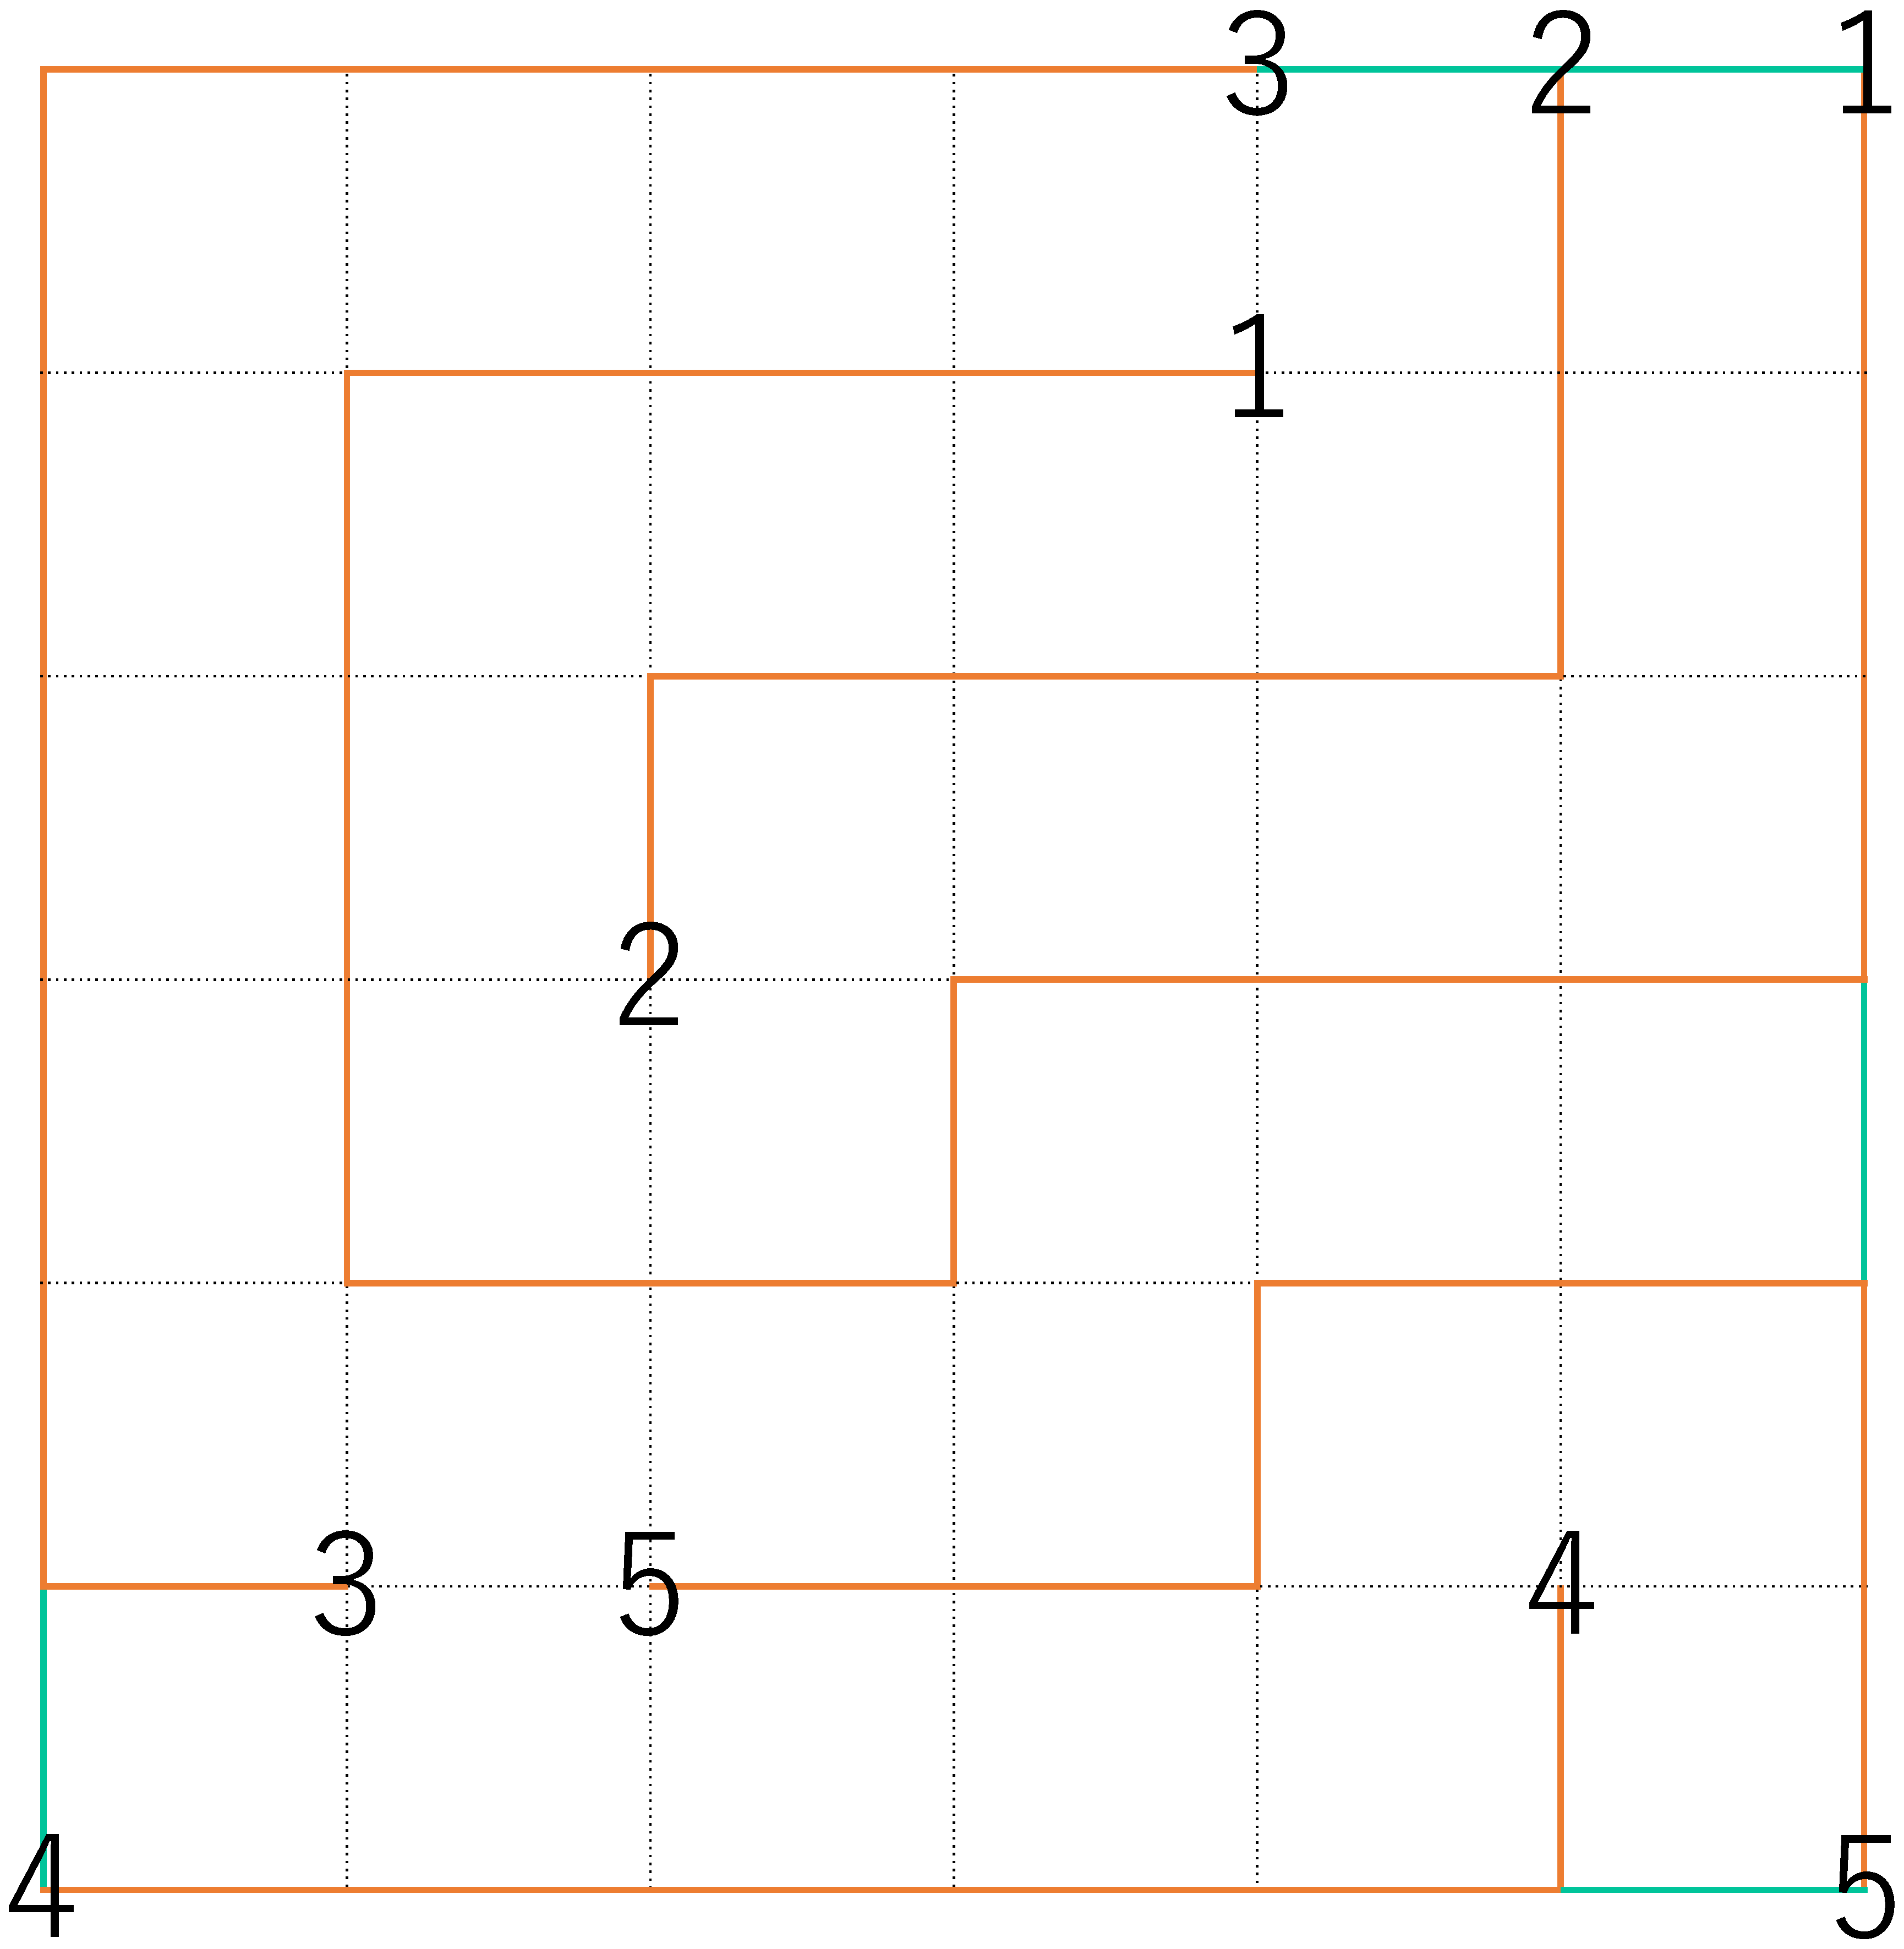
\includegraphics[width=0.85\linewidth,clip]{fig/NumberLink.eps}
  \caption{ナンバーリンクの完成盤面(リプレイス前)}
  \label{figure:NumberLink}
\end{clearpagefigure}

\begin{clearpagefigure}
  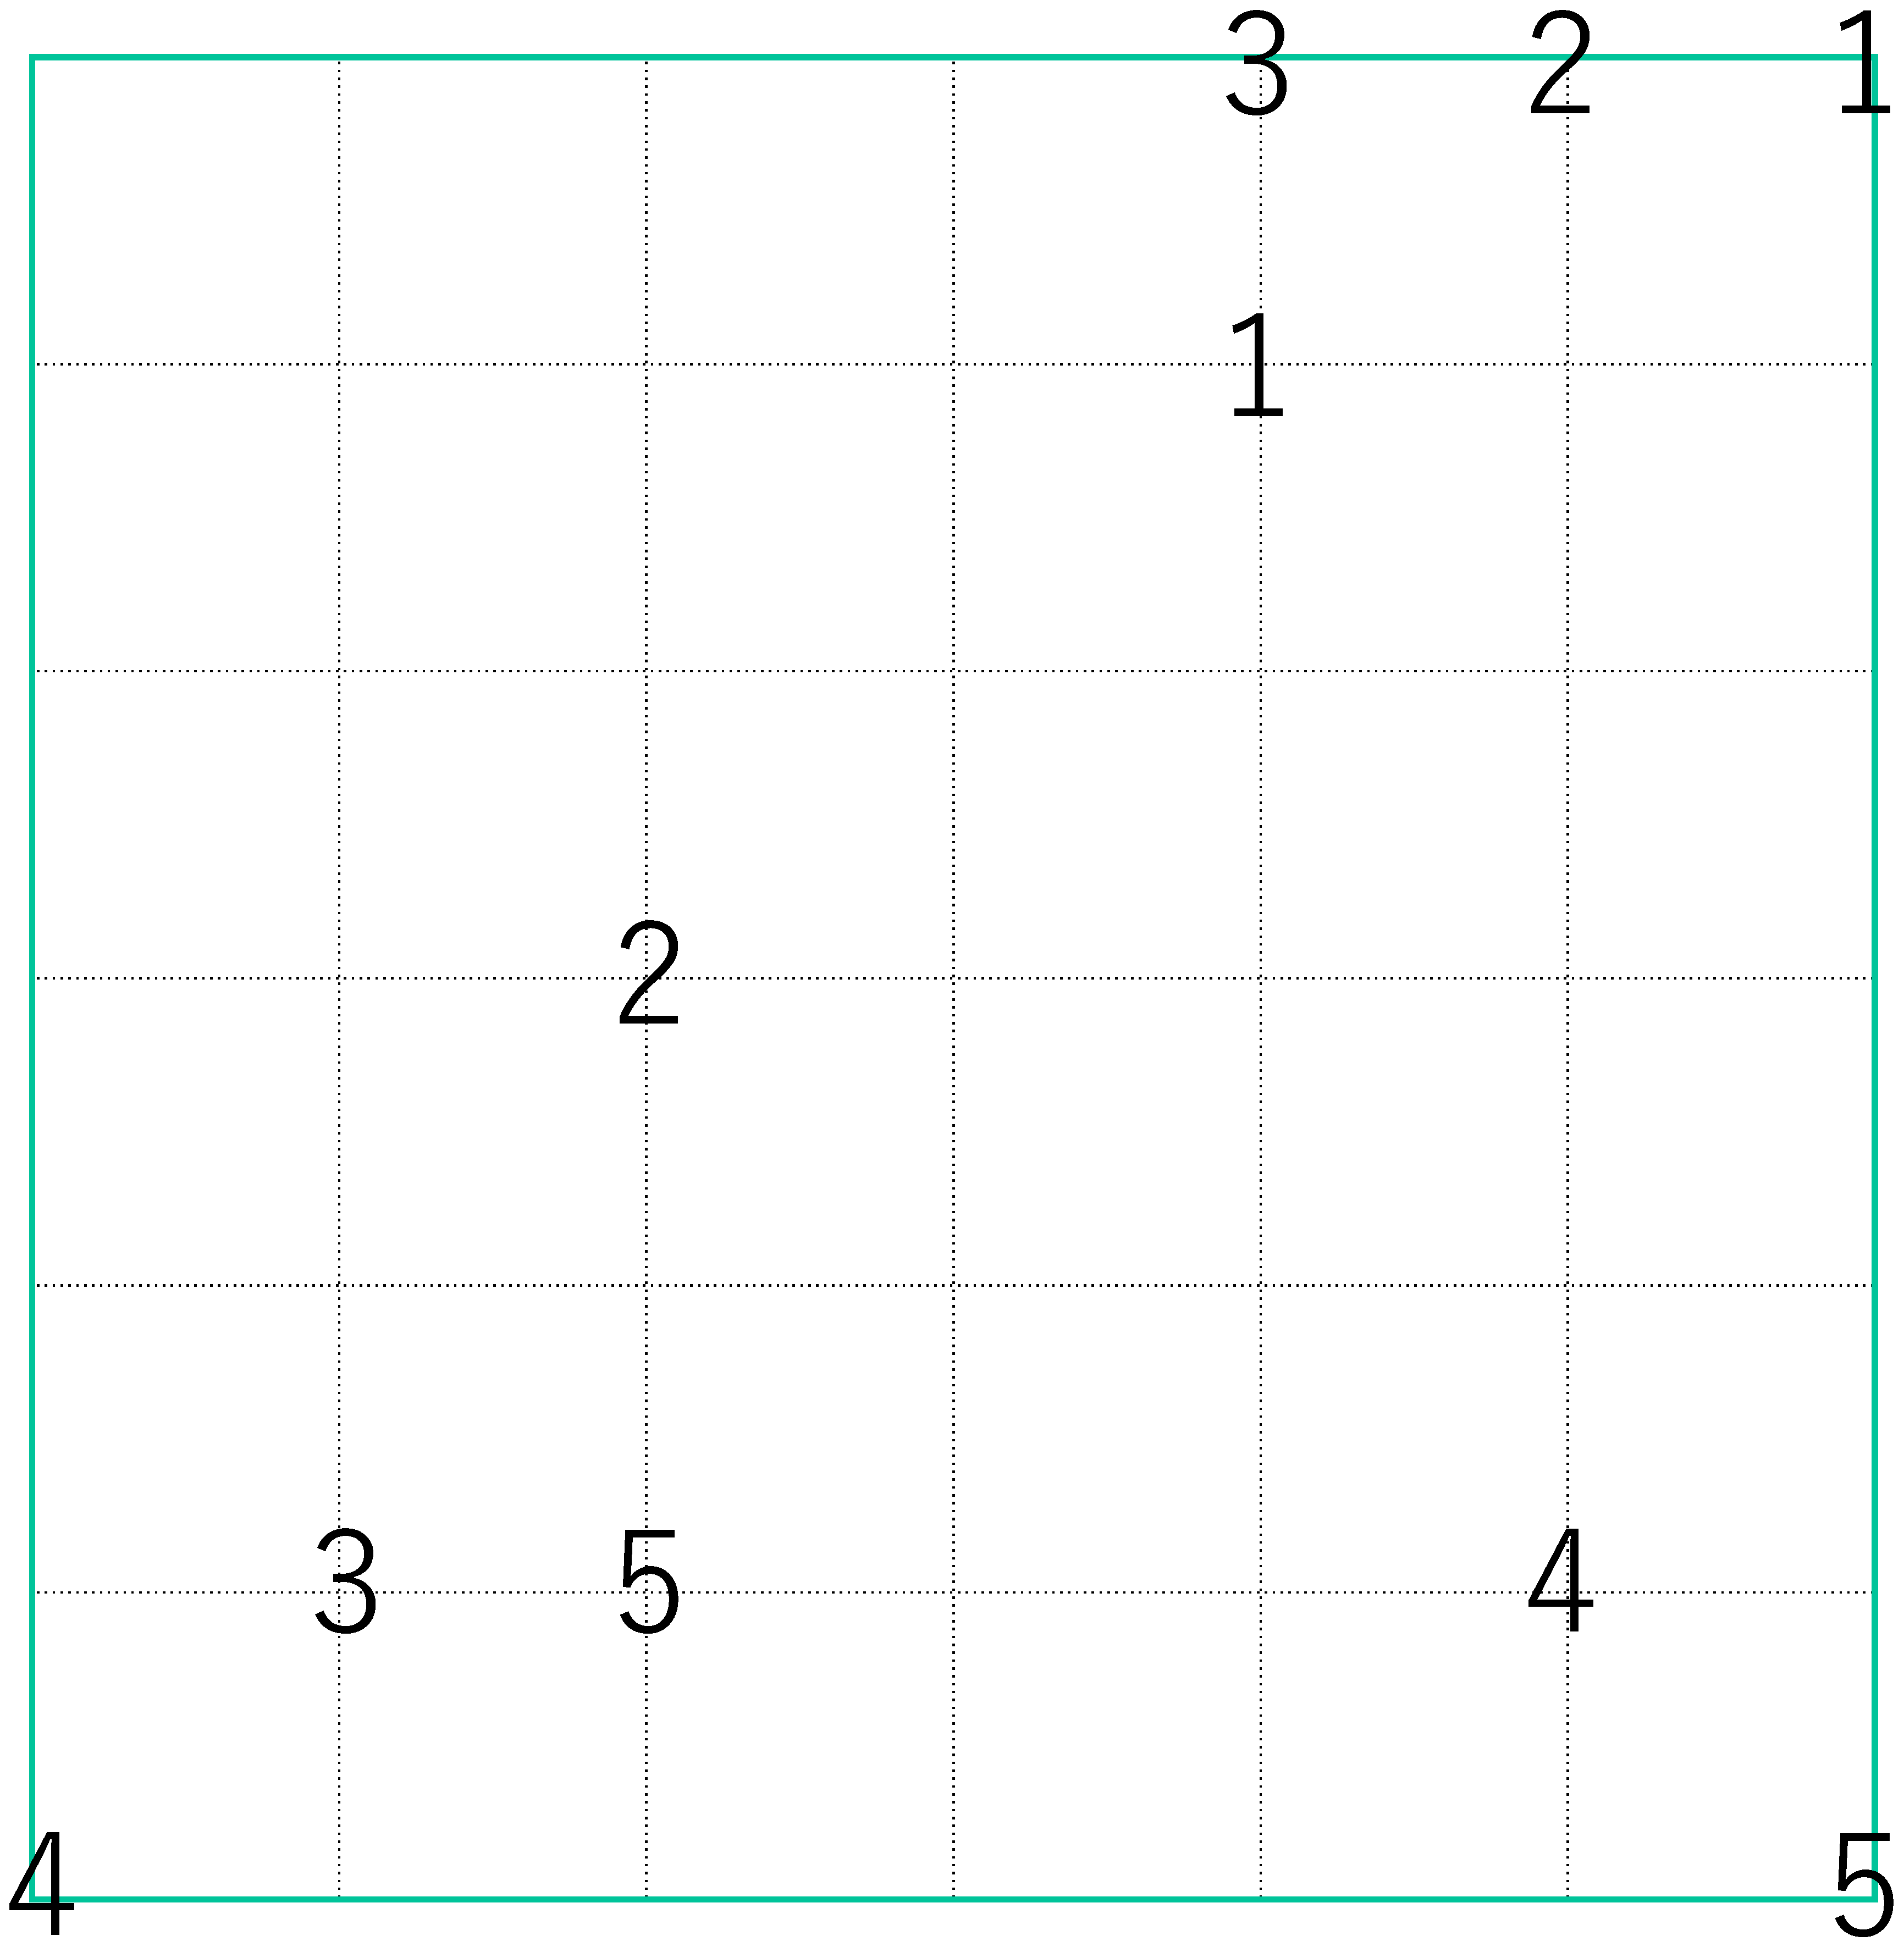
\includegraphics[width=0.85\linewidth,clip]{fig/NumberLinkQuestion.eps}
  \caption{ナンバーリンクの非完成盤面(リプレイス前)}
  \label{figure:NumberLinkQuestion}
\end{clearpagefigure}

\begin{clearpagefigure}
  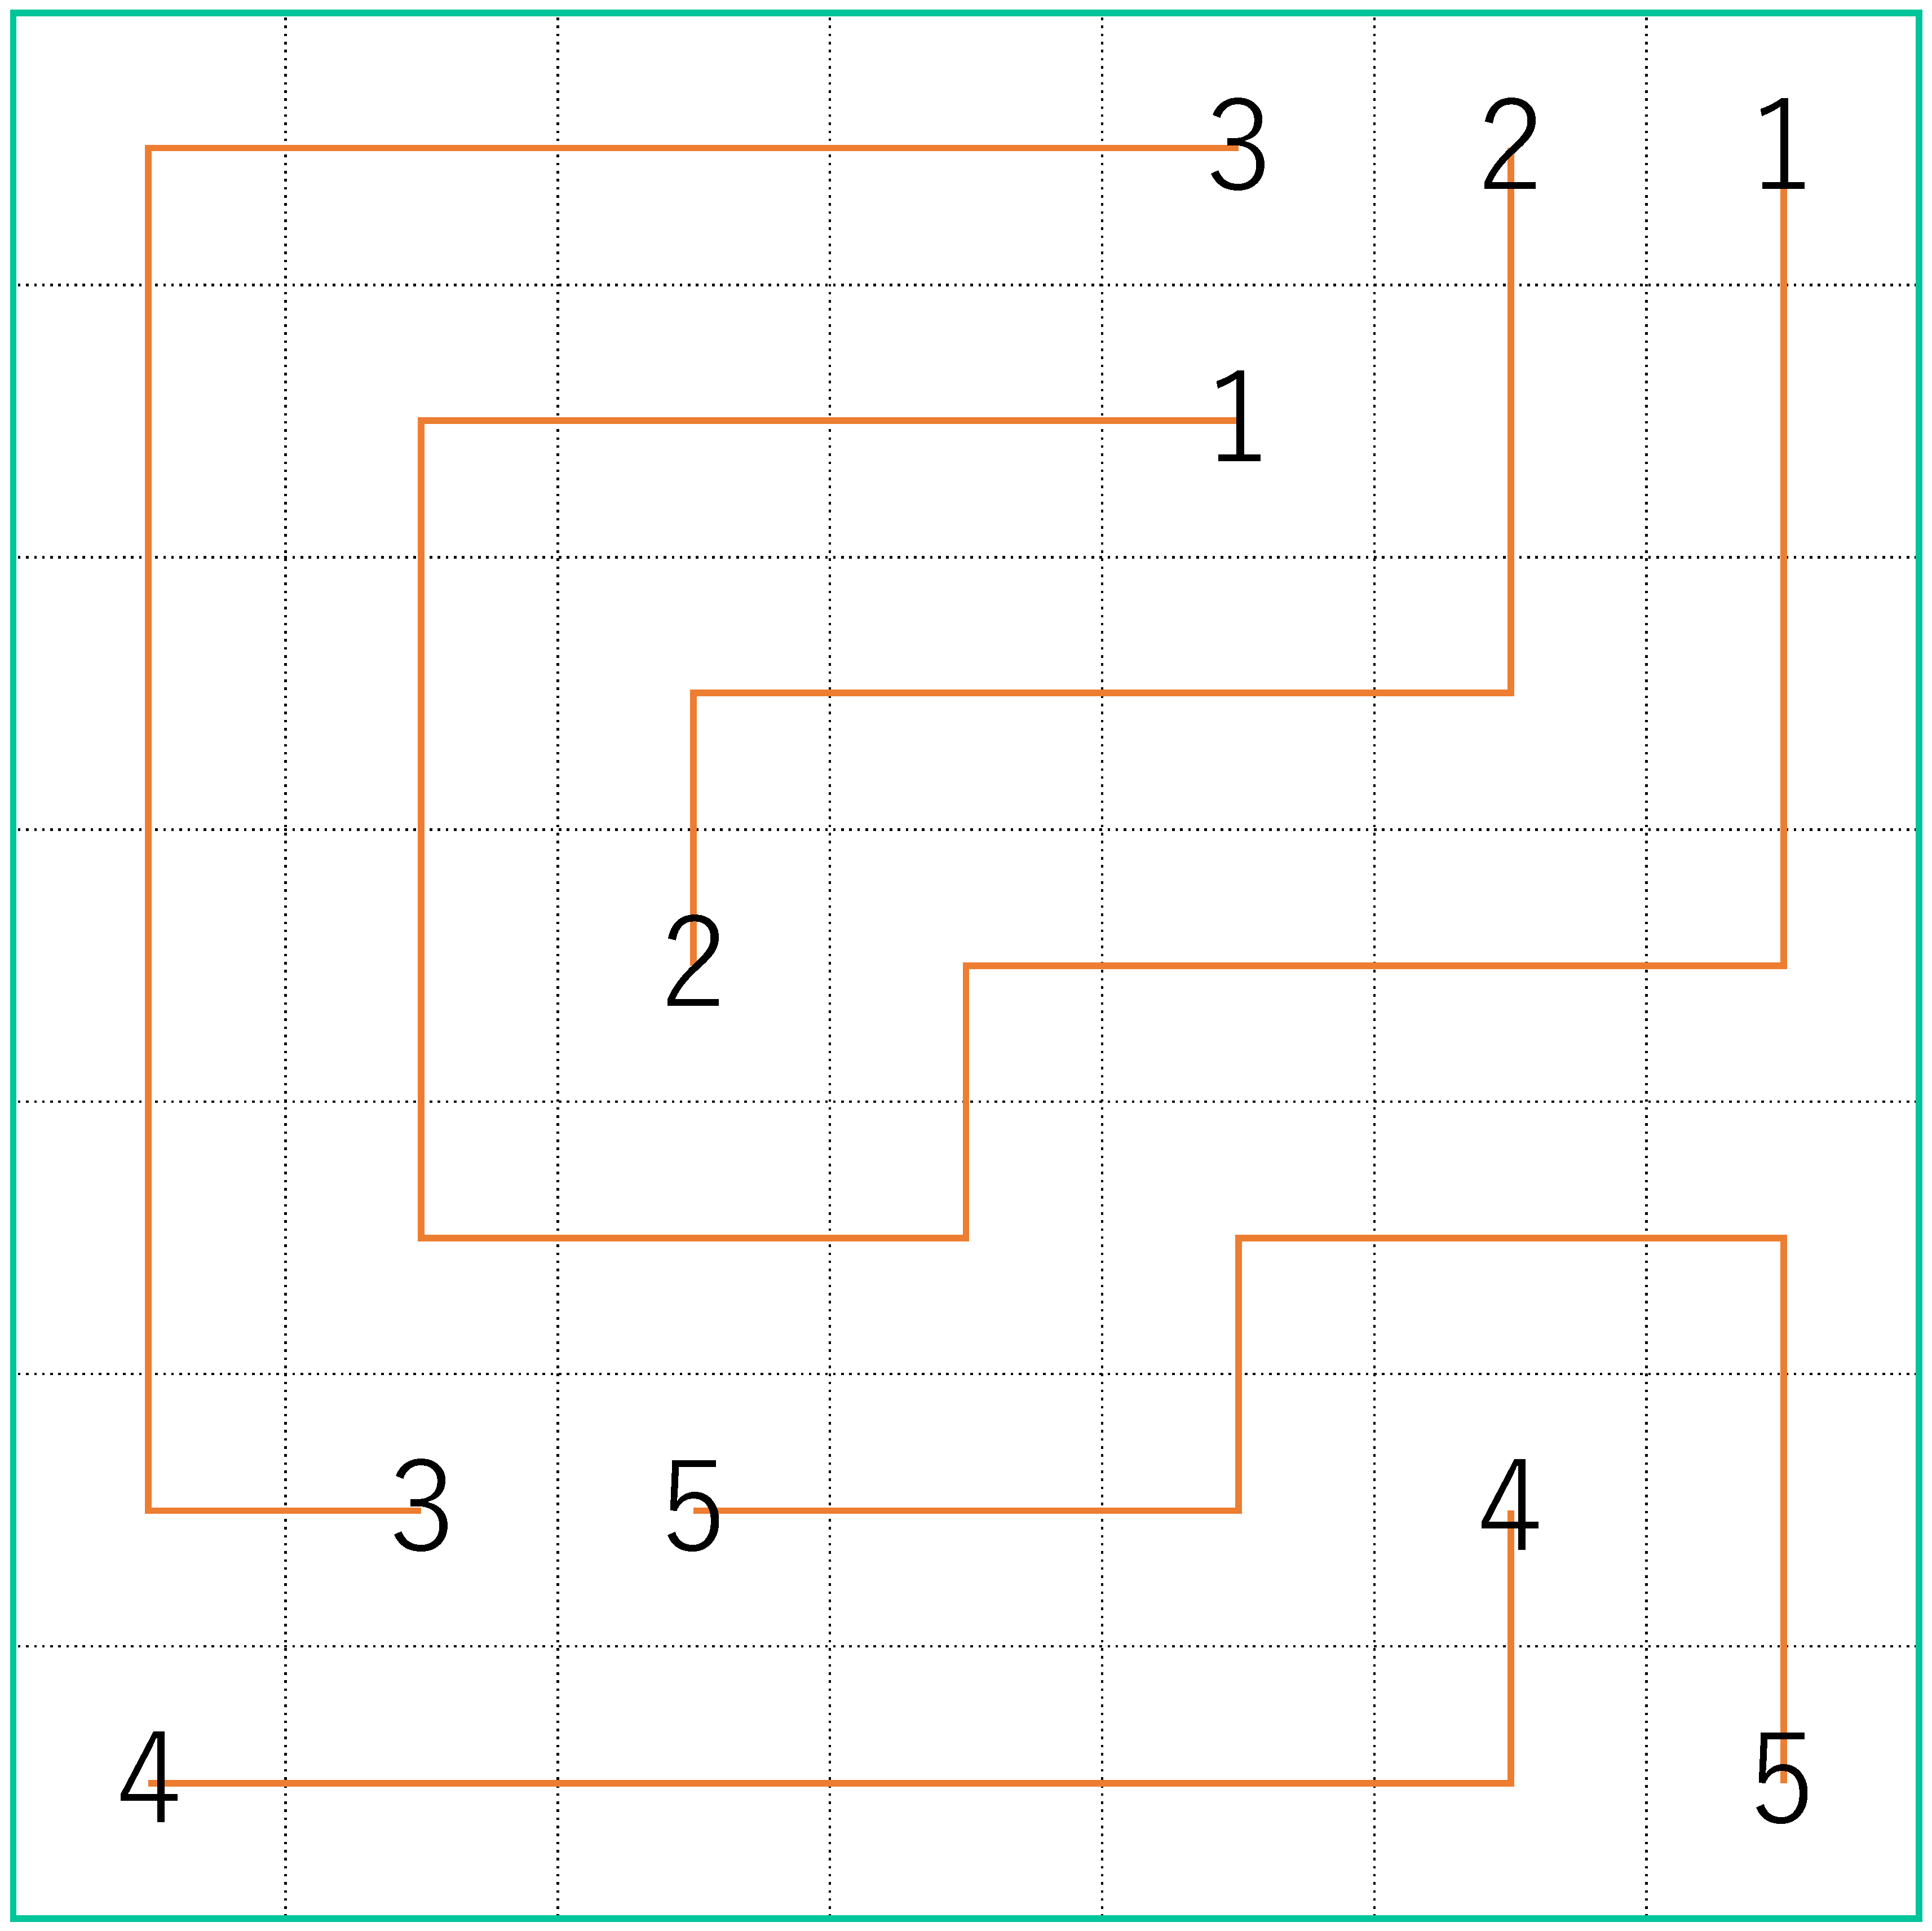
\includegraphics[width=0.85\linewidth,clip]{fig/NumberLinkReplace.eps}
  \caption{ナンバーリンクの完成盤面(リプレイス後)}
  \label{figure:NumberLinkReplace}
\end{clearpagefigure}

\begin{clearpagefigure}
  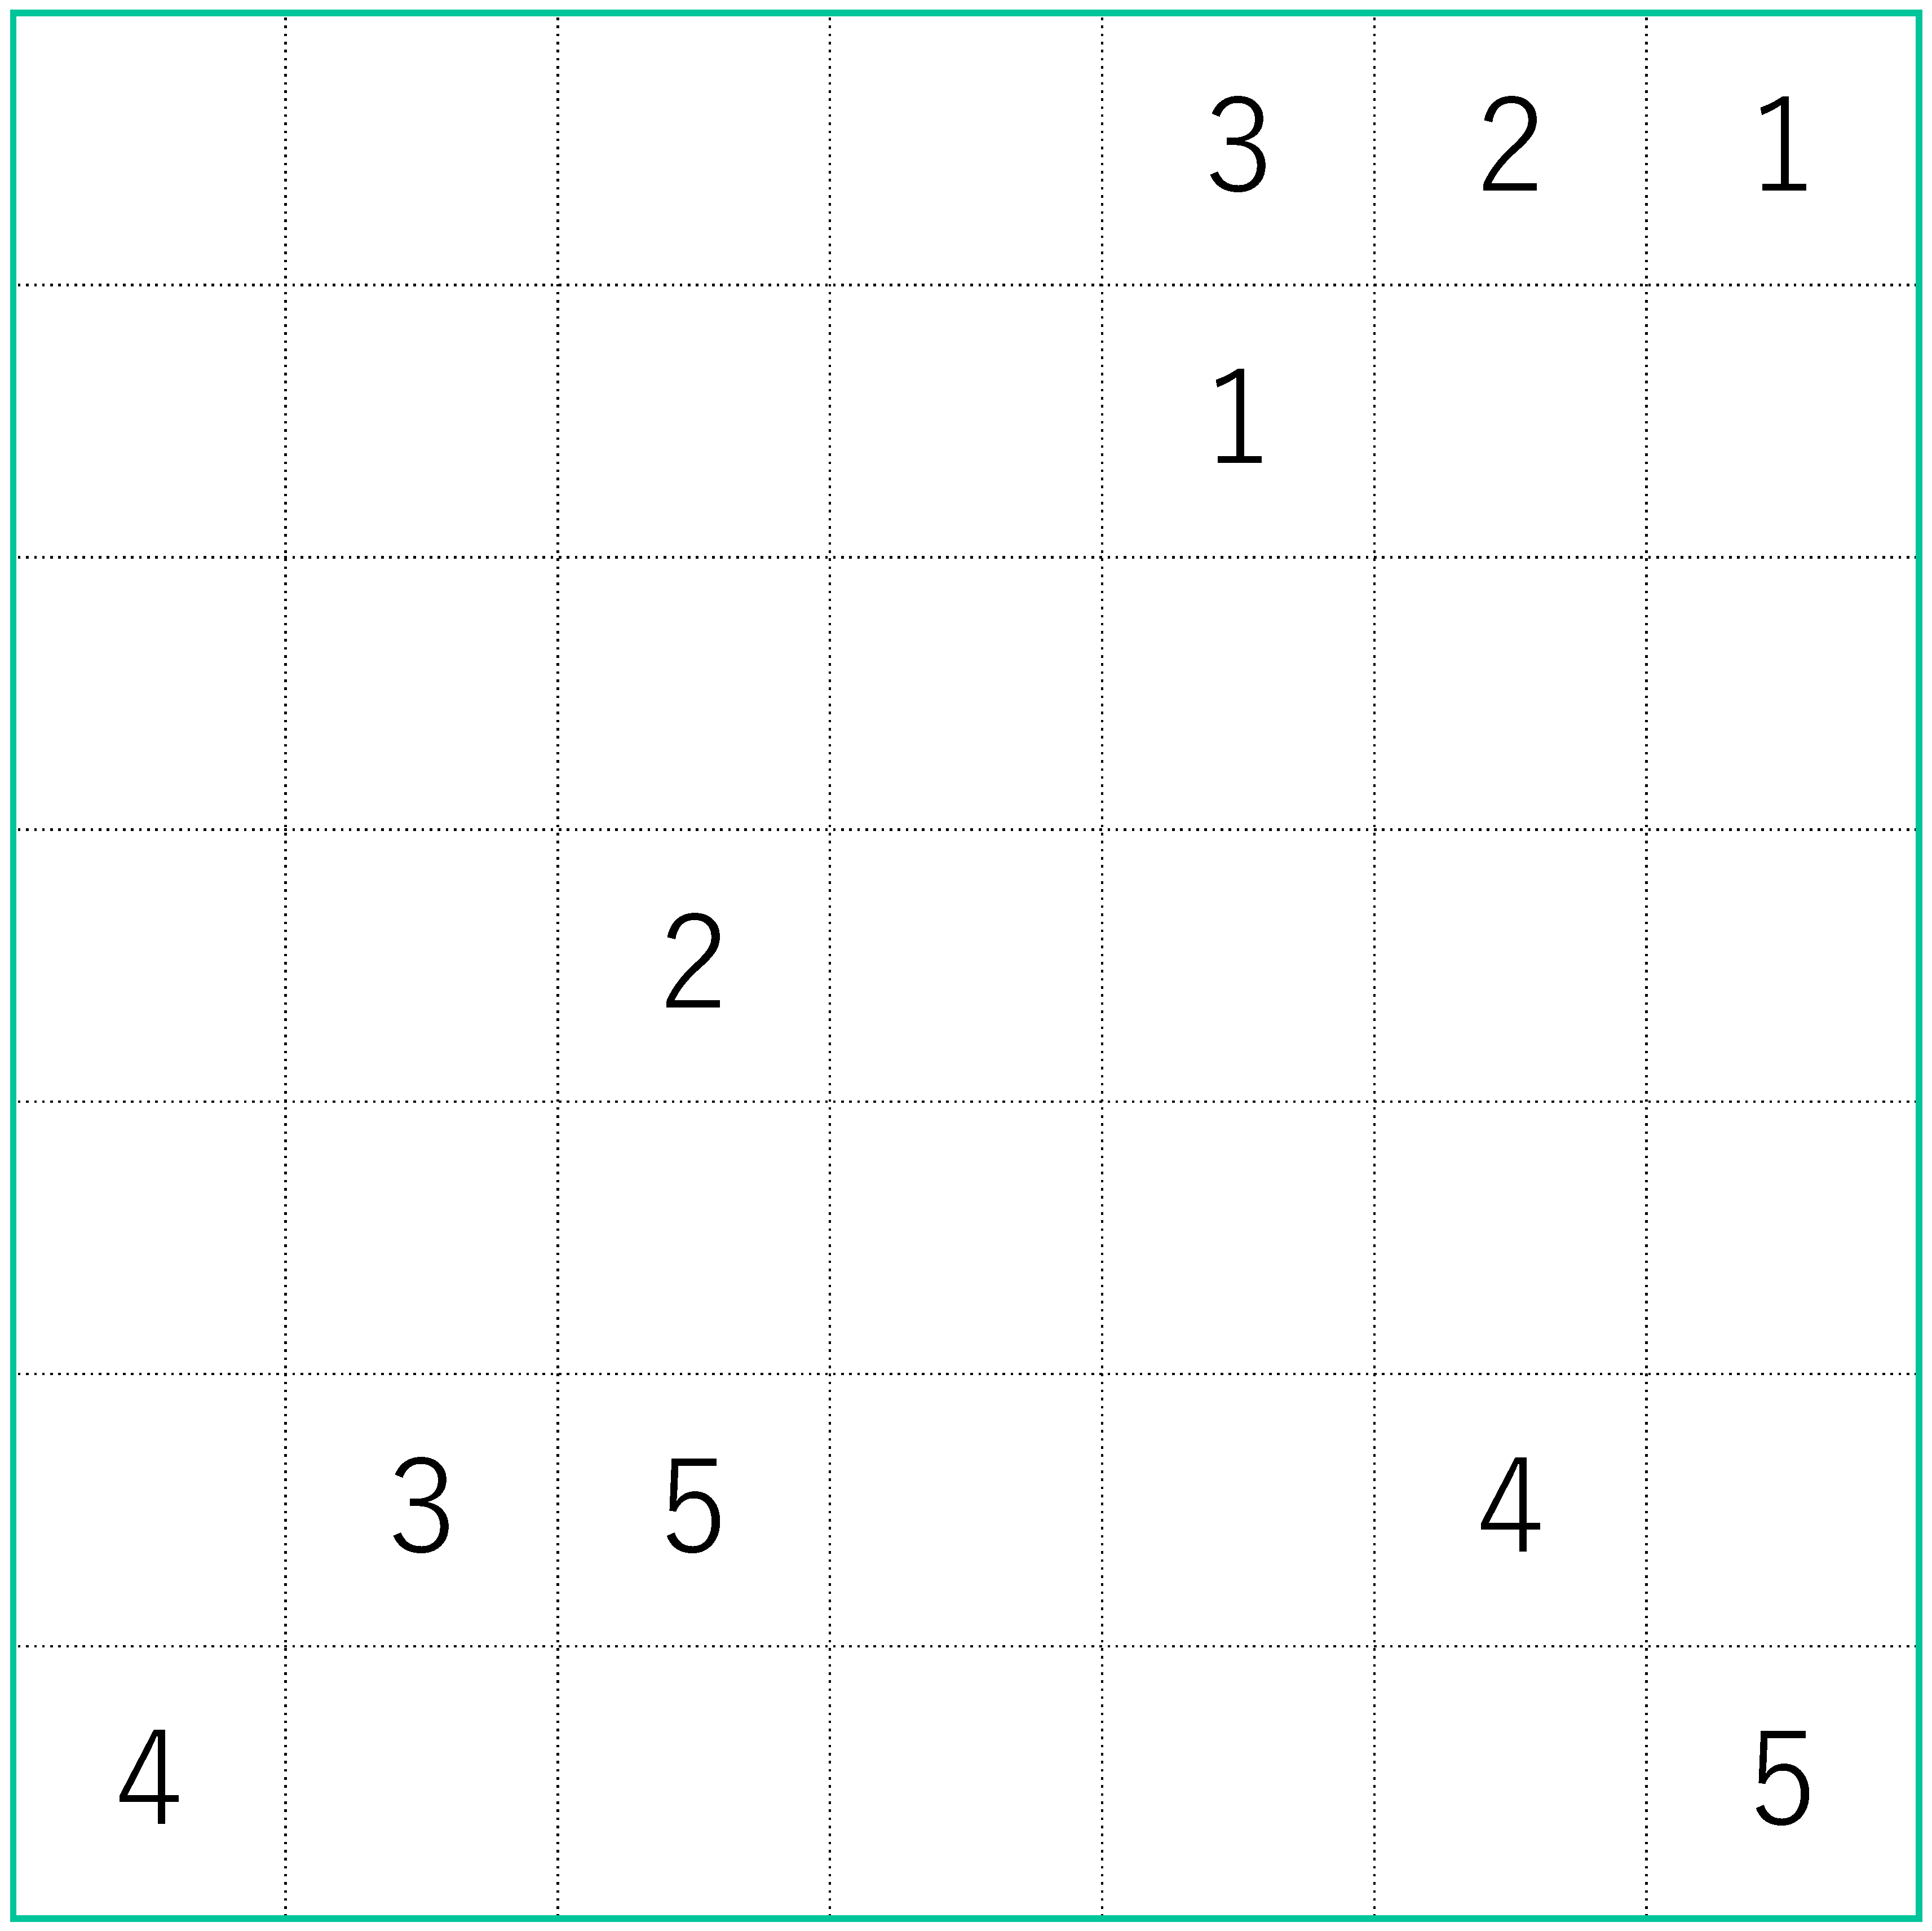
\includegraphics[width=0.85\linewidth,clip]{fig/NumberLinkQuestionReplace.eps}
  \caption{ナンバーリンクの完成盤面(リプレイス後)}
  \label{figure:NumberLinkQuestionReplace}
\end{clearpagefigure}

\begin{clearpagefigure}
  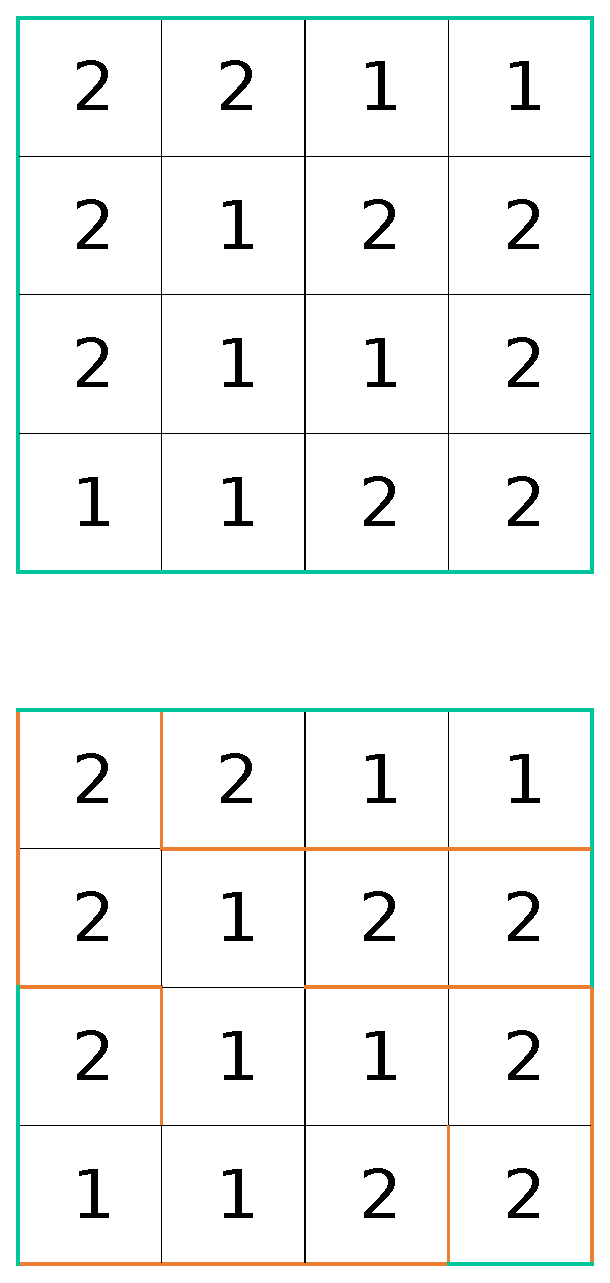
\includegraphics[width=0.5\linewidth,clip]{fig/NewPuzzleRule.eps}
  \caption{新しく作成したパズルルール. 上が非完成盤面, 下が完成盤面. }
  \label{figure:NewPuzzleRule}
\end{clearpagefigure}

\chapter{結言}
\cref{chapter:Definition}では, サイズ$m\times n$の平面グリッドを与えた際に, 種々の数学的定義を行うことでパズルルールが定義できることを主張した. また, パズルルールを構成する中枢を担う\textit{conditions}の具体的な構成方法について\cref{section:ConcreteConditions}で説明を行った. \cref{chapter:Demonstration}では本研究におけるパズルルールの定義を用いることで, 既存のパズルルールを数学的に記述することを可能にすることを示した. さらに, \cref{section:ConcreteConditions}で説明した\textit{conditions}の構成方法を用いることによって, 新規のパズルルールを作成できることを示した.

このパズルルールの定義を用いることで, 既存, 新規にかかわらずパズルルールの数学的記述ができる. さらに, \textit{conditions}の性質の分類, 抽象化を行うことでパズルルールの体系的な分類が期待される. これらが実現すればパズルルールの機械的な作成, あるいは自動作成が期待できる. 本論文中で触れた, \cref{theorem:AutoGeneration}の適用条件を明確にできれば, 自動作成したパズルルールの具体的な問題を作成できるため, 商業用ゲームへの移植が実現できる.

今後の展望として, まず本文中で触れたように\cref{theorem:AutoGeneration}の適用範囲について明確にすることが挙げられる. これに成功すれば, その適用範囲を満たしている\textit{codomain}と\textit{conditions}を満たす完成盤面を一つ考えることができれば, それは問題の存在と同値になり, より実用的になることが期待される.

さらに, ペンシルパズルの体系的な難易度評価の研究が挙げられる. 研究段階では\textit{codomain}とHIの選び方によりパズルルールの難易度が変わることが定性的に分かっている. Komiya-Kotani-Korekawa\cite{Komiya2010}はペンシルパズルの難易度を"Solution Path"という概念を考案し, 体系的に難易度評価を行っている. しかしこれはあるパズルルールが存在したときの問題の難易度であり, パズルルール自体の難易度を測る指標ではない. パズルルール自体の難易度を\textit{codomain}とHIから定量的に算出する方法があれば, 自動作成されたパズルルールがより実用的になることが期待される.

他に, ペンシルパズルの定義を本論文では平面グリッドとしたが, 実際には六角形グリッドであったり, 球体上にグリッドを配置したパズルも考えることができる. 研究段階で, 平面グリッドであるための必要十分条件が「盤面$B$において, あるグラフ$G_z$が存在したとき, $G_z \ni \forall p(i,j)$, $\text{cross}(p(i,j))\le3$」であると予想されている. この制約を外すことによって, 立体形状にグリッドを配置したパズルを体系的に考えることができると期待される.
\chapter{タイトル}
%\label{chap:chapter5}


\newcounter{pagenumberbody}
\setcounter{pagenumberbody}{\value{page}}

\appendix
\setcounter{page}{1}
\renewcommand{\thepage}{A--\arabic{page}}
\chapter{タイトル}
%\label{chap:appendixA}



% \renewcommand{\thepage}{\arabic{page}}
% \setcounter{page}{\value{pagenumberbody}}

\setcounter{page}{1}
\renewcommand{\thepage}{B--\arabic{page}}
\backmatter
\bibliography{reference} % reference.bibの読み込み

\chapter{謝辞}
%\label{chap:acknowledgement}



\end{document}
